	%%% LaTeX Template: Designer's CV
%%%
%%% Source: http://www.howtotex.com/
%%% Feel free to distribute this template, but please keep the referal to HowToTeX.com.
%%% Date: March 2012


%%%%%%%%%%%%%%%%%%%%%%%%%%%%%%%%%%%%%
% Document properties and packages
%%%%%%%%%%%%%%%%%%%%%%%%%%%%%%%%%%%%%
\documentclass[a4paper,11pt,final]{memoir}

% misc
\renewcommand{\familydefault}{bch}	% font
\pagestyle{empty}					% no pagenumbering
\setlength{\parindent}{0pt}			% no paragraph indentation

\usepackage[T1]{fontenc}
\usepackage[utf8]{inputenc}
% required packages (add your own)
\usepackage{flowfram}										% column layout
\usepackage[top=1cm,left=1cm,right=1cm,bottom=1cm]{geometry}% margins
\usepackage{graphicx}										% figures
\usepackage{url}											% URLs
\usepackage[usenames,dvipsnames]{xcolor}					% color
\usepackage{multicol}										% columns env.
	\setlength{\multicolsep}{0pt}
\usepackage{paralist}										% compact lists
\usepackage{tikz}
\usepackage{hyperref}
\hypersetup{colorlinks,citecolor=black,filecolor=black,linkcolor=black,urlcolor=black} % pour mettre les liens en noirs, sans cadre
\usepackage[english]{babel}

%%%%%%%%%%%%%%%%%%%%%%%%%%%%%%%%%%%%%
% Create column layout
%%%%%%%%%%%%%%%%%%%%%%%%%%%%%%%%%%%%%
% define length commands
\setlength{\vcolumnsep}{\baselineskip}
\setlength{\columnsep}{\vcolumnsep}

% frame setup (flowfram package)
% left frame
\newflowframe{0.2\textwidth}{\textheight}{0pt}{0pt}[left]
	\newlength{\LeftMainSep}
	\setlength{\LeftMainSep}{0.2\textwidth}
	\addtolength{\LeftMainSep}{1\columnsep}
 
% small static frame for the vertical line
\newstaticframe{1.5pt}{\textheight}{\LeftMainSep}{0pt}
 
% content of the static frame
\begin{staticcontents}{1}
\hfill
\tikz{%
	\draw[loosely dotted,color=RoyalBlue,line width=1.5pt,yshift=0]
	(0,0) -- (0,\textheight);}%
\hfill\mbox{}
\end{staticcontents}
 
% right frame
\addtolength{\LeftMainSep}{1.5pt}
\addtolength{\LeftMainSep}{1\columnsep}
\newflowframe{0.7\textwidth}{\textheight}{\LeftMainSep}{0pt}[main01]


%%%%%%%%%%%%%%%%%%%%%%%%%%%%%%%%%%%%%
% define macros (for convience)
%%%%%%%%%%%%%%%%%%%%%%%%%%%%%%%%%%%%%
\newcommand{\Sep}{\vspace{1.5em}}
\newcommand{\SmallSep}{\vspace{0.5em}}

\newenvironment{AboutMe}
	{\ignorespaces\textbf{\color{RoyalBlue} About me}}
	{\Sep\ignorespacesafterend}
	
\newcommand{\CVSection}[1]
	{\Large\textbf{#1}\par
	\SmallSep\normalsize\normalfont}

\newcommand{\CVItem}[1]
	{\textbf{\color{RoyalBlue} #1}\normalsize\normalfont}
	
\newcommand{\city}[1]
	{{\small\textbf{#1}}\normalsize\normalfont}
	
\newcommand{\SkillSection}[1]
	{\small{\textbf{#1\\}}\normalfont\footnotesize}
	
\newcommand{\SkillItem}[1]
	{\textbf{\color{RoyalBlue} #1}\normalfont\\}
	
%%%%%%%%%%%%%%%%%%%%%%%%%%%%%%%%%%%%%
% Begin document
%%%%%%%%%%%%%%%%%%%%%%%%%%%%%%%%%%%%%
\begin{document}

% Left frame
%%%%%%%%%%%%%%%%%%%%
% Photo
\begin{figure}
	\hfill
	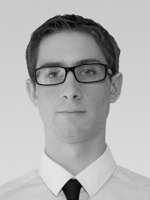
\includegraphics[width=0.6\columnwidth]{IMG_7936-Modifier_cv}
	\vspace{-0.5cm}
\end{figure}

% Personnal Infos
\begin{flushright}\small
	Romain \textsc{Reignier} \\
	%\url{romain.reignier@edu.supmeca.fr}  \\
	\href{mailto:romain.reignier@edu.supmeca.fr}{\nolinkurl{romain.reignier@edu.supmeca.fr}}\\
	+33609521618 \\
	23 years old
\end{flushright}%\normalsize

% Languages
\SkillSection{Languages}
\SkillItem{English}
Advanced level\\
TOEIC: 920 points\\
\SkillItem{Spanish}
Baccalaureat level\\
\SkillItem{German}
Beginner
\SmallSep

% Engineering
\SkillSection{Engineering}
Mechnanics\\
Resistance of the materials\\
%Materials\\
Digital methods\\
Algorithmic\\
Database\\
Thermal transferts\\
Automatic\\
Servo-system\\
Design of Systems\\
Analysis of mechanisms\\
Communication
\SmallSep

% Computer Skills
\SkillSection{Computer Skills}
\SkillItem{Word Processing Programs}
Word, Excel, Access, PowerPoint, LaTeX\\
\SkillItem{CAD}
CATIA V5, SolidWorks, ADAMS\\
%\SkillItem{Mathematics}
%Matlab, Maple\\
\SkillItem{Programming}
C/C++, Pyhton, Matlab, LabView, Maple, OpenCV\\
microcontrollers: Arduino, AVR, PIC, ARM\\
%embedded computing: Arduino \& AVR\\
\SkillItem{Web Development}
HTML5, CSS3, PHP, MySQL\\
\SkillItem{Image Editing}
Photoshop, Lightroom, Illustrator, Gimp, Inkscape
\SmallSep

% Sports
\SkillSection{Sports}
Cycling\\
MTB\\
Running\\
Swimming
\SmallSep

% Hobbies
\SkillSection{Hobbies}
Photography\\
Electronics\\
Gardening / Farming\\
General mechanics\\
First level diploma in aeronautics
\SmallSep

% Travels
\SkillSection{Travels}
Malaysia, Singapore, Togo, Netherlands, Germany, Czech Republic, Austria, Switzerland
\framebreak


% Right frame
%%%%%%%%%%%%%%%%%%%%
\Huge\bfseries {\color{RoyalBlue} Romain \textsc{Reignier}} \\
\Large\bfseries  Student in Mechanical \& Robotics Engineering \\

\normalsize\normalfont

% About me
\begin{AboutMe}
Je veux faire des tracteurs :p
\end{AboutMe}

% Education
\CVSection{Education}

\CVItem{2013 - present, University of Toulon} - \city{La Garde, Var}\\
Master Degree on Command \& Vision.
\SmallSep

\CVItem{2012 - present, Supmeca Engineering School} - \city{La Garde, Var}\\
An engineering course focusing in mechanics with Robotics and Mecatronics.
\SmallSep

\CVItem{2009 - 2012, CPGE Victor Hugo} - \city{Caen, Normandy}\\
Physics Sciences of Engineer (PSI).\\
Highly selective classes to prepare for the competitive exams to the Grandes Ecoles.
\SmallSep

\CVItem{2006 - 2009, Scientific Baccalaureat} - \city{Valognes, Normandy}\\
Secondary School diploma in Sciences, specialized in Physics.
%With Honors.
\Sep

% Experience
\CVSection{Experience}
\CVItem{September 2013 - January 2014, R\&D CLAAS Tractor} - \city{Vélizy, Yvelines}\\
Assistant engineer internship.\\
Work with the HVAC expert on the project to improve the AC of the K07 cabin.
Analysis of data from simulations and tests.
\SmallSep

\CVItem{January 2013, DCNS} - \city{Cherbourg, Normandy}\\
Operator internship.\\
Work with numerical machine tools in the construction workshop of French nuclear
submarines.
\SmallSep

\CVItem{From 2006 to 2012}\\
Various jobs\ldots
\Sep

\CVSection{Projects \& Associations}
\CVItem{CRIS}\\
The robotic club of Supmeca: conception, building and programmation of
robots for the national contest: Eurobot. %Score of 41 and 81 in 2012 and 2013
\SmallSep

\CVItem{Supwave}\\
Responsible of the electronics in an autonomous sailboat.
\SmallSep

\CVItem{Aerocorp}
Responsible of the internal electronics and actuators of a model aircraft.
\SmallSep

\CVItem{Supmeca Sans Frontières}\\
Humanitarian association which has the aim of bringing water to a Togolese orphanage.
\SmallSep

\CVItem{Scouts et Guides de France}\\
Boyscout for 8 years.\\
Humanitarian project in Togo in August 2013.

%\CVSection{Skills}
% \CVItem{Platforms}
%\begin{multicols}{3}
% \begin{compactitem}[\color{RoyalBlue}$\circ$]
% 	\item Lorem 
% 	\item Ipsum 
% \end{compactitem}
%\end{multicols}
%\SmallSep

% \CVItem{Computer software}
% \begin{multicols}{3}
% \begin{compactitem}[\color{RoyalBlue}$\circ$]
% 	\item Lorem 
% 	\item Ipsum 
% 	\item Dolor 
% 	\item Sit 
% 	\item Amet
% 	\item Consectetur 
% 	\item Adipiscing 
% 	\item Elit
% 	\item \ldots
% \end{compactitem}
% \end{multicols}
% \Sep 
% 
% \CVSection{Something other}
% Lorem ipsum dolor sit amet, consectetur adipiscing elit. Vivamus vel bibendum metus. Proin rutrum pharetra molestie. Cras sollicitudin nulla nec leo lobortis in tristique purus pretium. Ut eu felis nulla. Pellentesque condimentum justo ut ligula feugiat nec facilisis tellus ultricies. Nullam sit amet dictum ipsum. Sed lacus neque, hendrerit eu rhoncus nec, pellentesque vitae sem.
% 
% \clearpage
% \framebreak
% \framebreak
% 
% \CVSection{Something else}
% Lorem ipsum dolor sit amet, consectetur adipiscing elit. Vivamus vel bibendum metus. Proin rutrum pharetra molestie. Cras sollicitudin nulla nec leo lobortis in tristique purus pretium. Ut eu felis nulla. Pellentesque condimentum justo ut ligula feugiat nec facilisis tellus ultricies. Nullam sit amet dictum ipsum. Sed lacus neque, hendrerit eu rhoncus nec, pellentesque vitae sem.
% \Sep
% 
% % References
% \CVSection{References}
% References upon request.

%%%%%%%%%%%%%%%%%%%%%%%%%%%%%%%%%%%%%
% End document
%%%%%%%%%%%%%%%%%%%%%%%%%%%%%%%%%%%%%
\end{document}
